\documentclass{beamer}
\usetheme{Marburg}

\usepackage[ansinew]{inputenc}
\usepackage[ngerman]{babel}
\usepackage{xcolor}
\usepackage{fancybox}


\usepackage{graphicx}
\usepackage{icomma,units}
\usepackage{amsfonts,amsmath,amssymb}
\usepackage{enumerate}
\usepackage{booktabs}
\usepackage{colortbl}


%Einstellung aus dem Pr�sentationstemplate
\beamersetuncovermixins{\opaqueness<1>{25}}{\opaqueness<2->{15}}

%Farbdefinitionen
\definecolor{dunkelgrau.80}{gray}{0.20}
\definecolor{dunkelgrau.60}{gray}{0.40}
\definecolor{hellgrau}{rgb}{0.95,0.95,0.95}
\definecolor{Dschungelgr\"{u}n}{cmyk}{0.99,0,0.52,0.2}
\definecolor{midblue}{rgb}{0.173,0.212,0.597}



\begin{document}

\title{Region Oberrhein -- Rhin Sup\'{e}rieur}   
\author{Pascal Bernhard} 
\date{\today}
\titlegraphic{
\includegraphics[width=3.8cm,height=0.9cm]{Logo_Trinationale_Metropolregion_Oberrhein.png}}
\logo{\includegraphics[scale=0.14]{logo-SF}}

%%%-------------------------------------------------------------------------------------------------------------------%%%

\begin{frame}
\titlepage
\end{frame}

%%%-------------------------------------------------------------------------------------------------------------------%%%

\begin{frame}
\frametitle{Inhalt}\tableofcontents
\end{frame}

%%%-------------------------------------------------------------------------------------------------------------------%%%

\section{Geografische Lage} 

%%%

\begin{frame}\frametitle{Die Region Oberrhein in Europa} 

\begin{center}
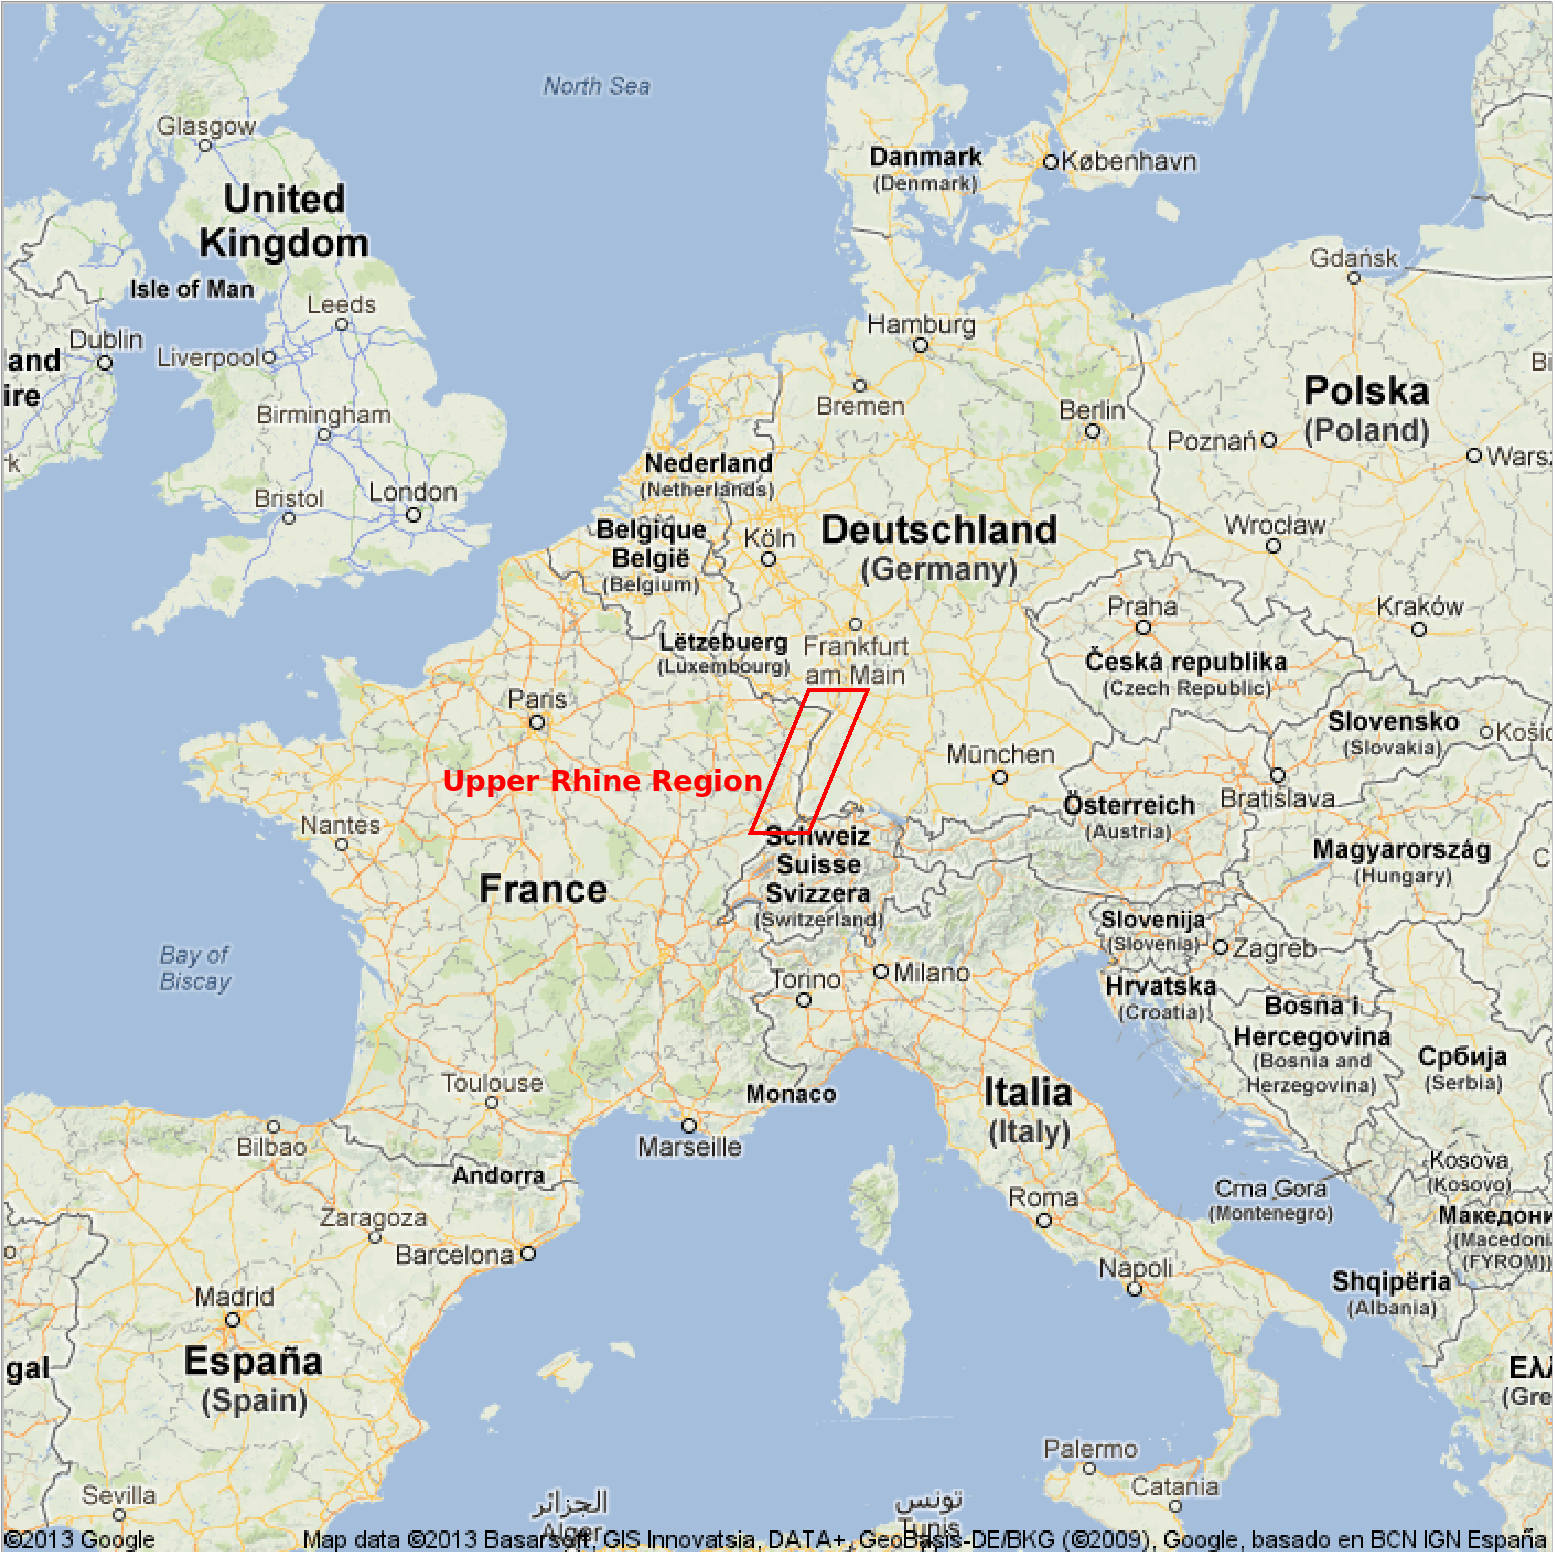
\includegraphics[width=7.03cm,height=7.0cm]{GoogleMaps_Western-Central-Europe.png} 
\end{center}

\end{frame}


%%%-------------------------------------------------------------------------------------------------------------------%%%

\begin{frame}\frametitle{Teil der europ�ischen Wirtschaftsachse} 

\begin{center}
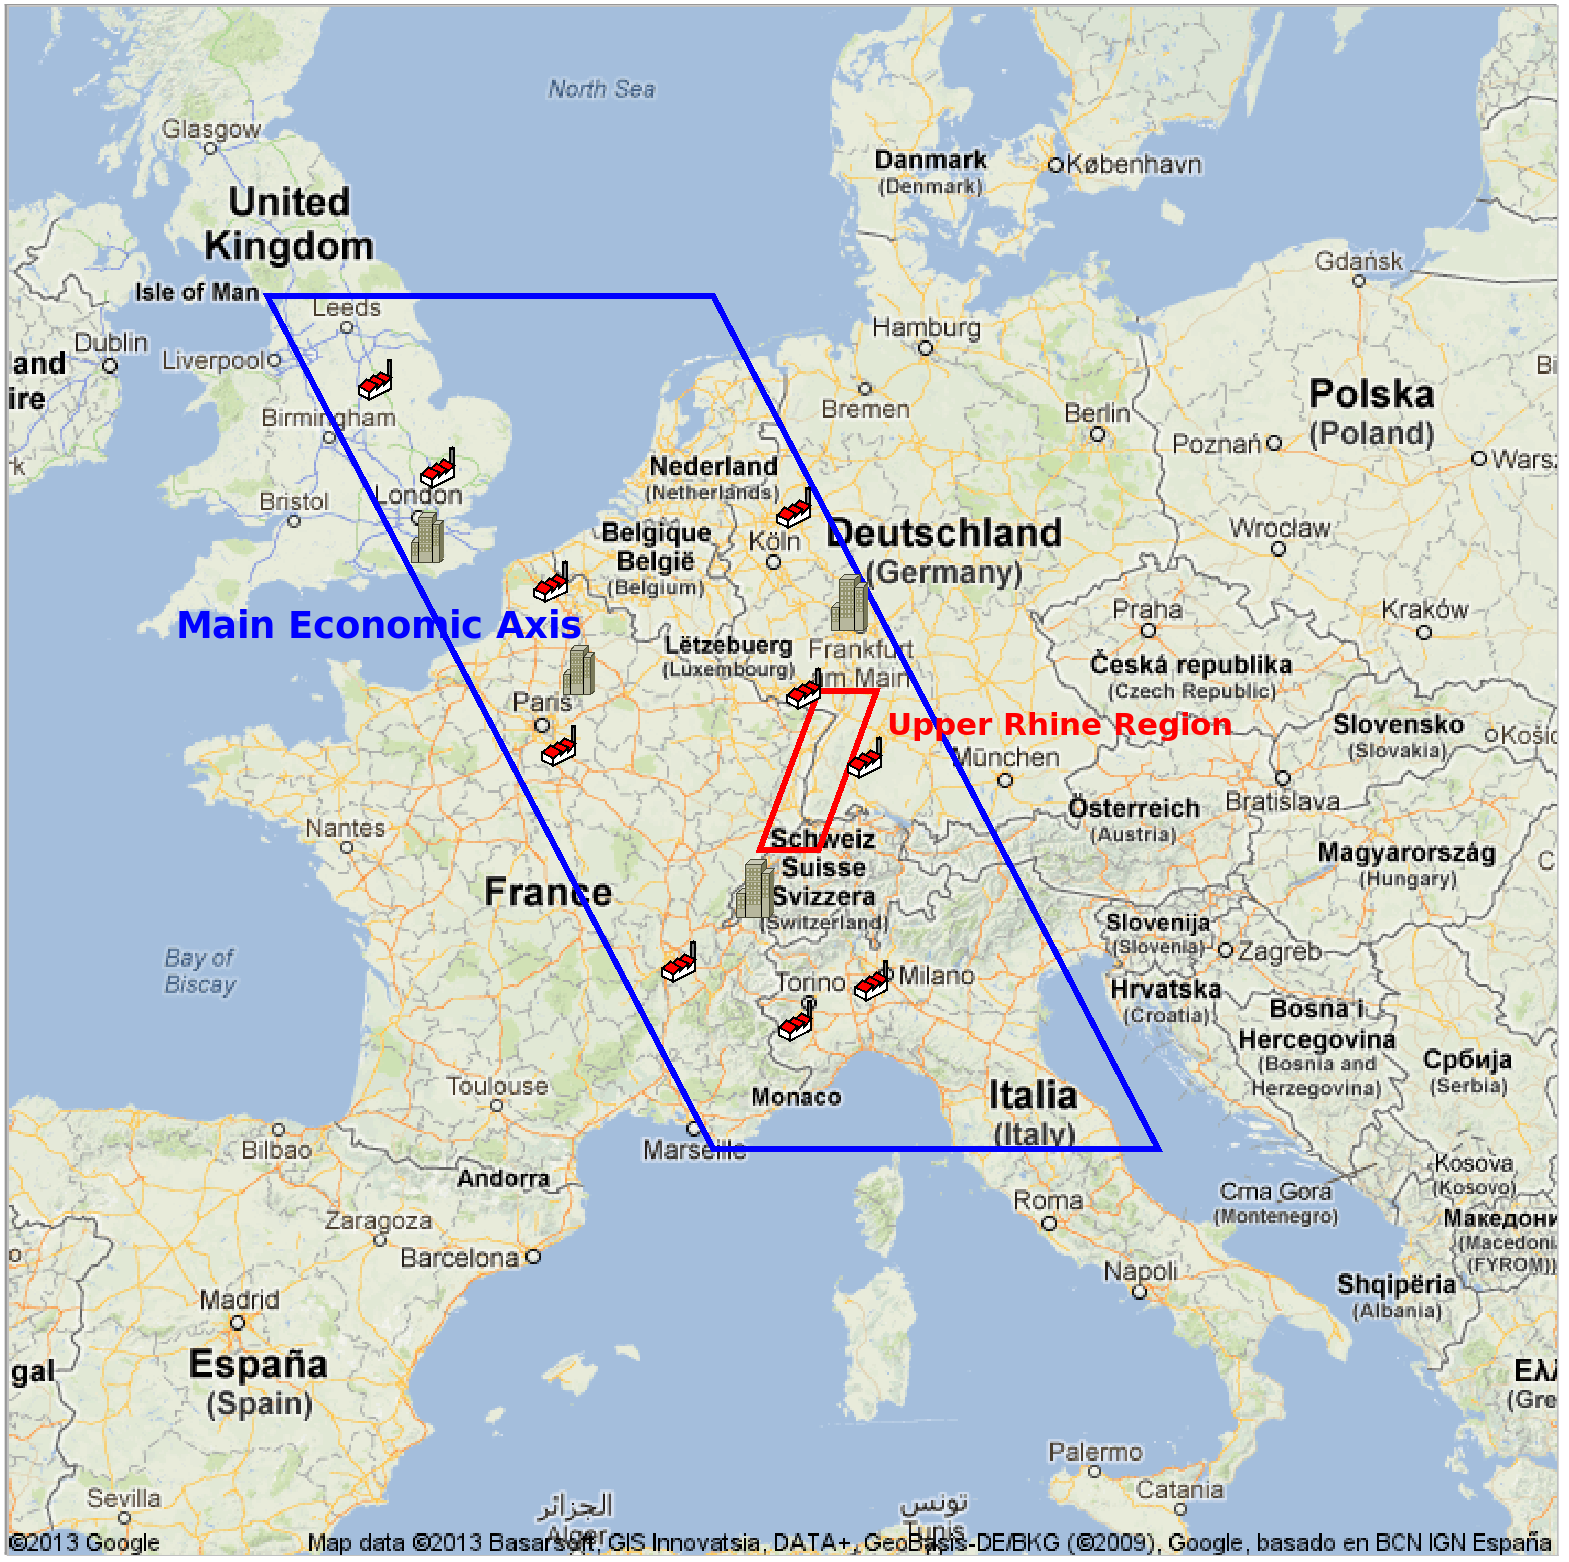
\includegraphics[width=7.03cm,height=7.0cm]{GoogleMaps_Western-Central-Europe_Parallelogramm_Pixbuff.png} 
\end{center}

\end{frame}


%%%-------------------------------------------------------------------------------------------------------------------%%%


\begin{frame}\frametitle{Lokale Topografie} 

\begin{center}
\includegraphics[width=5.53cm,height=8.0cm]{Oberrheinkonferenz_Mandatsgebiet.png} 
\end{center}

\end{frame}

%%%-------------------------------------------------------------------------------------------------------------------%%%


\begin{frame}\frametitle{Geografische Merkmale}


  \begin{itemize}
    \item Teil der Hauptachse wirtschaftlicher Aktivit�t\\
	 $\Rightarrow$ Nord-S�d--Verkehrstrom (\textsl{Rotterdam-Genua})\\
	 $\Rightarrow$ Bedarf an Verkehrsinfrastruktur

    

    \item Fluss Rhein als Grenze und Wasserweg

    

    \item \textbf{Touristenattraktionen:} Vogesen und Schwarzwald sowie St�dte Strasbourg \& Freiburg 
    

    \item dezentrale Bev�lkerungsstruktur aber hohe Bev�lkerungsdichte!\\
 	 $\Rightarrow$ keine Gro�st�dte
   \end{itemize}

\end{frame}



%%%-------------------------------------------------------------------------------------------------------------------%%%

\section{Trinationale Zusammenarbeit} 

\subsection{Gemeinsame Themen}

\begin{frame}\frametitle{Politikfelder}

  \begin{itemize}
    \item Umweltprobleme
      \begin{enumerate}
	\item Luftverschmutzung
	\item Wassermanagement am Rhein
      \end{enumerate}

      

    \item Forschung \& Bildung\\
 	 $\Rightarrow$ F�rderung Zweisprachigkeit (Deutsch-Franz�sisch)
  \end{itemize} 

\end{frame}

%%%-------------------------------------------------------------------------------------------------------------------%%%

\begin{frame}\frametitle{Politikfelder}

  \begin{itemize}
    \item Infrastruktur
      \begin{enumerate}
	\item Verkehrsinfrastruktur (\textsl{Trans European Networks -- TEN})
	\item Integration des �ffentlichen Nahverkehrs
      \end{enumerate}

      

    \item Wirtschaftsentwicklung
      \begin{enumerate}
	\item Vermarktung von ``Oberrhein'' als eigene Marke
	\item F�rderung erneuerbarer Energien
	\item Zusammenarbeit bei Ausbildung (Handwerk, berufliche Weiterbildung)
      \end{enumerate}
  \end{itemize} 

\end{frame}


%%%-------------------------------------------------------------------------------------------------------------------%%%


\begin{frame}\frametitle{Oberrheinkonferenz}

\begin{center}
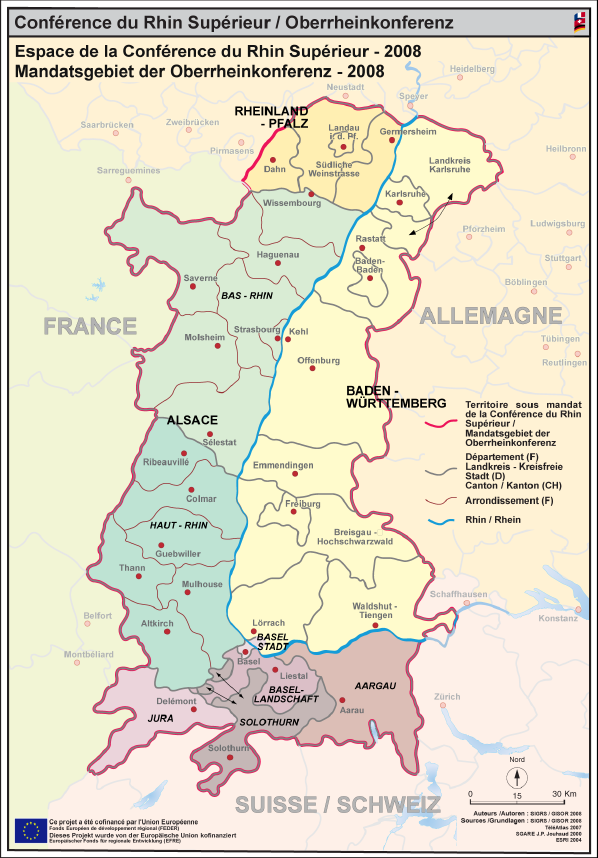
\includegraphics[width=5.53cm,height=8.0cm]{Mandatsgebiet_Oberrheinkonferenz.png} 
\end{center}

\end{frame}


%%%-------------------------------------------------------------------------------------------------------------------%%%
\section{Regionale Institutionen} 

\subsection{Zusammenarbeit nationaler Verwaltungen}

\begin{frame}
\frametitle{Oberrheinkonferenz}
 
  \begin{itemize}
    \item Idee hat Ursprung bilateralen Vertr�gen zwischen Deutschland und Frankreich (\textsl{\'{E}liys\'{e}e-Vertrag}: 1963)
    
    \item  Deutsche, Franz�sische \& Schweizer Delegation (Beamte)
    
    \item Arbeitsgruppen f�r spezifische Politikbereiche (Experten aus regionalen Verwaltungen)\\
    $\Rightarrow$ \textbf{Ziel:} Austausch von Informationen auf technischem Niveau
  \end{itemize}


\end{frame}



%%%-------------------------------------------------------------------------------------------------------------------%%%



\subsection{Koordination Regionalpolitik}

\begin{frame}
\frametitle{Oberrheinrat}

  \begin{itemize}
    \item gegr�ndet 1997
    
    \item 4 Delegationen aus Frankreich (\textcolor{dunkelgrau.60}{\emph{R\'{e}gion Alsace}: 26 Delegation}), Deutschland (\textcolor{dunkelgrau.60}{\emph{Baden-W�rtemberg}: 26 Delegierte \& \emph{Rheinland-Pfalz}: 8 Delegierte}), und Schweiz (\textcolor{dunkelgrau.60}{\emph{Basel-Stadt, Basel-Landschaft, Solothurn, Aargau}: 11 Delegierte})\\ 
    
    $\Rightarrow$ \textbf{Ziel:} Institution f�r Informationsaustausch auf politischer Ebene und Politikkoordination 
  \end{itemize}


\end{frame}

%%%-------------------------------------------------------------------------------------------------------------------%%%
\section{Fazit}

\begin{frame}
\frametitle {Abschlie�ende Bemerkungen}

\begin{block}{Regionale Institutionen}
   \emph{Oberrheinkonferenz} und \emph{Oberrheinrat} haben KEINE legislative Kompetenzen, auch KEINE Ausf�hrungsvollmachten
\end{block}

  

\begin{block}{Projekte}
    Wenig Bedeutung f�r Bev�lkerung:\\
    \emph{Zweisprachiges Schulbuch zu regionaler Geschichter, gemeinsamer Museumspass, Webseite zur Luftqualit�t, Expertengruppen \& Workshops}
\end{block}


\end{frame}





\end{document}


%%%%%%%%%%%%%%%%%%%%%%%%%%%%Versuch eine Tabelle zu erstellen%%%%%%%%%%%%%%%%%%%%%%%%%%%%%%%%%%%%%%%%%%%%%%%%%%%%%%%%%%%%

\setlength{\tabcolsep}{25pt}
\renewcommand{\arraystretch}{2.5}

\begin{tabular}{l c c c c}
  \toprule[2pt]	\rowcolor{hellgrau}
  Region & Area & Population & Unemployment & GDP \\
  \hline
  \hline
  Alsace \\
  \cmidrule[0.5pt]{2-5}
  Rheinland-Pfalz \\ 
  \cmidrule[0.5pt]{2-5}
  Baden-W�rtemberg \\
  \cmidrule[0.5pt]{2-5}
  North-West Switzerland \\
  \bottomrule[2pt]

\end{tabular}


